\documentclass{article}
\usepackage{amsmath}
\usepackage{mathptmx}
\usepackage{tikz}
\usepackage{pgfplots}
\usepackage{tkz-fct}
\usetikzlibrary{angles, quotes}
\usetikzlibrary{arrows.meta, arrows}
\usepgfplotslibrary{polar}
\usepgfplotslibrary{fillbetween}
\usetikzlibrary{external}
\tikzexternalize[prefix={external/}]

\tikzset{
    export as png/.style={
        external/system call/.add={}{
            && convert -density #1 -transparent white "\image.pdf" "\image.png"
        },
    },
    export as png/.default={200},
}

\DeclareSymbolFont{symbolsb}{OMS}{cmsy}{m}{n}
\SetSymbolFont{symbolsb}{bold}{OMS}{cmsy}{b}{n}
\DeclareSymbolFontAlphabet{\mathcal}{symbolsb}
\definecolor{myblue}{rgb}{0.067,0.529,0.871}
\definecolor{mypurple}{rgb}{0.859,0.071,0.525}
\definecolor{myred}{rgb}{1.0, 0.13, 0.32}
\definecolor{mygreen}{rgb}{0.01, 0.75, 0.24}
\definecolor{myblack}{gray}{0.5}
\definecolor{mygray}{gray}{0.7}

\def\req{\protect\rotatebox{90}{$\scriptstyle=$}}

\begin{document}

\tikzset{export as png}

\tikzsetnextfilename{area-entre-curvas-polares}
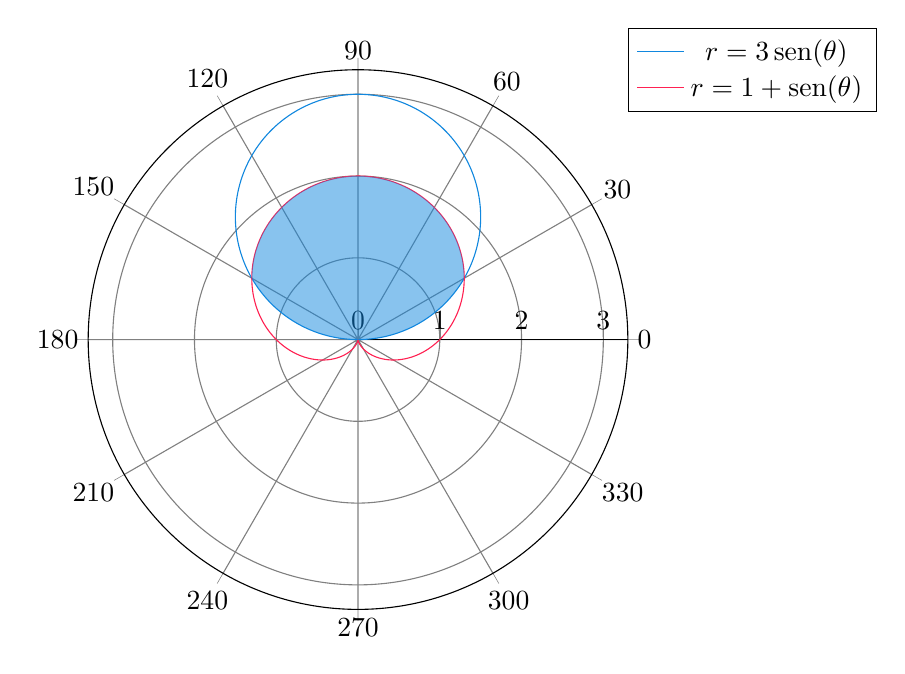
\begin{tikzpicture}
    \begin{polaraxis}[
        samples=360, % How many samples to take
        grid=major, % Display both major and minor grids
        major grid style={gray}, % Style for major grids
        %legend pos=north west, % Position of legend
        legend style={at={(1,1)},anchor=west},
    ]
    % First plot
    \addplot+[no marks, domain=180:360, myblue] {3*sin(\x)};
    \addlegendentry{$r = 3\operatorname{sen}(\theta)$}
    
    % Second plot
    \addplot+[no marks, domain=0:360, myred] {1 + sin(\x)};
    \addlegendentry{$r = 1 + \operatorname{sen}(\theta)$}
    
    % Fill between
    \addplot+[no marks, domain=0:180, fill=myblue, draw = none, opacity=0.5]{min(3*sin(\x), 1+sin(\x))}; 
    \end{polaraxis}
    \end{tikzpicture}
\end{document}


